\documentclass{article}
\usepackage{graphicx} % Required for inserting images
\usepackage{enumitem}
\usepackage[most]{tcolorbox}
\usepackage{amsmath}
\usepackage{float}
\newtheorem{property}{Property}
\usepackage{algorithm}
\usepackage{algpseudocode}



\title{M Tree}
\author{ricardo andre ulloa vega}
\date{June 2025}

\begin{document}
	
	\maketitle
	
	\section{Introduction}
		MM objects are characterized by means of relevant ``features``.
		
		\begin{enumerate}
		
		\item shapes
		\item  textures
		\item  patterns
		\item  colors for images
		\end{enumerate}
		
		The similarity queries. This process thus requires a \textit{distance function} to measure the similarity of feature values.
		
		The intrinsic multi-dimensional nature of features has suggested using spatial access methods \textbf{SAMs}, such \textbf{R-Tree}, however applicability of \textbf{SAMS} is limited by two major factors:
		\begin{enumerate}
			\item Objects are to be represented by means of feature values in a \textit{vector space} of dimensionality \textit{Dim}.
			\item The distance function has to be an $L_{p}$ norm, such as $L_{2}$ (Euclidean).
		\end{enumerate}
				
		\begin{tcolorbox}[colback=gray!10, colframe=gray!50, sharp corners, boxrule=0.5pt]
			Besides dynamicity, M-Tree does not dictate a specific algorithm to organized the indexed objects, rather only general principles are specified and detail are encapsulated in the implementation of maintenance methods.
			This approach makes the M-tree a \textbf{flexible structure}.
		\end{tcolorbox}

		
		
	\section{Preliminaries}
		Indexing a \textit{metric space}  aims to efficiently support similarity en queries.
		Formally, a \textit{metric space} is a pair $M = (D, d)$, where $D$ is a domain of features values and d is a total(distance).
					
			\begin{equation}
				\begin{aligned}
					 & (1) \quad d(O_x, O_y) = d(O_y, O_x)                                                          &  & \quad \text{(simetría)}               \\
					 & (2) \quad 0 < d(O_x, O_y) < \infty, \quad O_x \neq O_y, \quad \text{y} \quad d(O_x, O_x) = 0 &  & \quad \text{(no negatividad)}         \\
					 & (3) \quad d(O_x, O_y) \leq d(O_x, O_z) + d(O_z, O_y)                                         &  & \quad \text{(desigualdad triangular)}
				\end{aligned}
			\end{equation}

		
	\section{The M-tree}
	The M-tree organized the objects into fixed-size nodes, nodes can store up to M \textit{entries}, for each indexed DB object, one \textit{entry} whit the format.
	$$
		\text{entry}(O_{j}) = [O_{j}, \text{oid}(O_{j}), d(0_{j}, P(O_{j}))]
	$$
	This is stored in a \textbf{leaf node}.
	\begin{itemize}
		\item[$\cdot$] $O_{j}$ are the features values of the object (i.e, $O_{j} \in D$)
		\item[$\cdot$] $oid(O_{j})$ is the identifier of the object which resides on a separate data file. 
		\item[$\cdot$] $d(O_{j}, P(O_{j}))$ is the distance between $O_{j}$ and parent of $O_{j}$.
		
	\end{itemize}
	
	An entry in an no-leaf
	$$
	\text{entry}(O_{r}) = [O_{r},\ \text{ptr}(T(O_{r})),\ r(O_{r}),\ d(O_{r}, P(O_{r}))]
	$$

	\begin{itemize}
		\item[$\cdot$] $O_{r}$ also called \textit{routing object}.
		\item[$\cdot$] $r(O_{r})$ \textit{convering radius} 
		\item[$\cdot$] $T(O_{r})$ is the root of the sub-tree, also called \textit{covering tree}.
	\end{itemize}

	
	\begin{property}[Covering Radius]
		The covering radius \( r(O_r) \) of a routing object \( O_r \) defines the maximum distance from \( O_r \) to any object in its subtree \( T(O_r) \).
		\[
		r(O_r) = \max \big\lbrace d(O_r, O_j) \mid O_j \in T(O_r) \big\rbrace
		\]
	\end{property}
	
A routing object thus defines a region in a metric space \( M \), centered on \( O_r \) and with radius \(r(O_r)\) , and \(O_r\) is the parent of each object \(O_j\) stored in the node referenced by  \(\text{ptr}(T(O_r))\), i.e.\ \( O_r \equiv P(O_j) \) (see Figure~1).

	\begin{figure}[H]
		\centering
		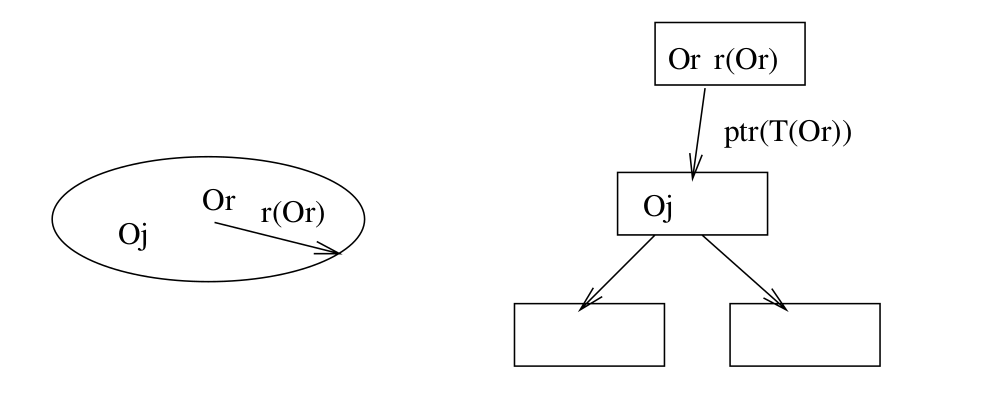
\includegraphics[width=0.6\textwidth]{../img/im1.png}
		\caption{A routing object, \( O_r \), has a covering radius, \( r(O_r) \), and references a covering tree, \( T(O_r) \).}
		\label{fig:routing_object}
	\end{figure}

	\subsection{How M-tree Grows}
	As any other dynamic balancer tree, M-tree grows in a bottom-up. You add objects to the node \(N\) until \(N\) reaches overflow then we need a new node \(N'\) at the same level of \(N\), partitioning the \(M+1\) entries among the two nodes, and then posting relevant information to the parent node, \(N_p\).
	When the root splits, a new root is created and the M-tree grows by one level.
	
		
		\begin{algorithm}
			\caption{\(\text{M-tree split}\)}
			\begin{algorithmic}[1]
				\Procedure{Split}{\(N:\text{M-tree node}; E:\text{M-tree_entry}\)}
				\State $f \gets 1$
				\For{$i = 1$ to $n$}
				\State $f \gets f \cdot i$
				\EndFor
				\State \Return $f$
				\EndProcedure
			\end{algorithmic}
		\end{algorithm}

\end{document}
